\documentclass[tikz,border=10pt]{standalone}
\usepackage{tikz}
\usetikzlibrary{arrows.meta}

% Kept byte-for-byte in sync with the inline TikZ block in
% 02-06-trading-problem-formulation.qmd (the PDF path). This file is the
% source for rl-loop.svg, which the HTML path serves -- if the two drift,
% the same Figure 1 renders differently in the PDF and on the web.

\begin{document}
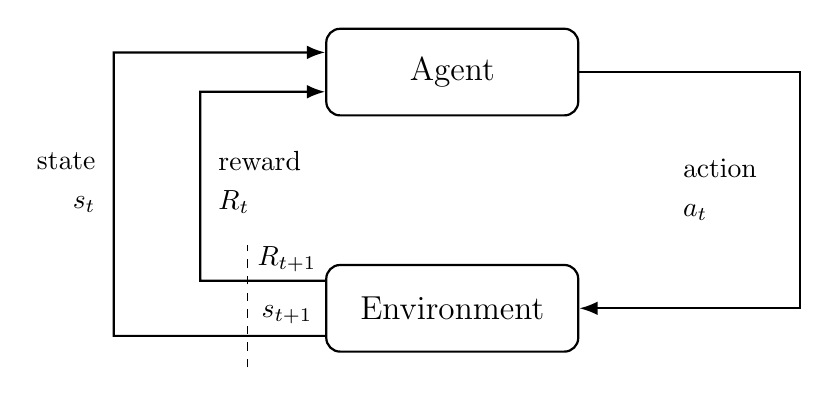
\begin{tikzpicture}[
  >=Latex,
  thick,
  box/.style={draw, rounded corners=5pt, minimum width=3.2cm, minimum height=1.1cm, font=\large}
]

\node[box] (agent) at (0, 3)  {Agent};
\node[box] (env)   at (0, 0)  {Environment};

% Right path (action)
\draw[->] (agent.east) -- ++(2.8,0) -- ++(0,-3) -- (env.east);
\node[right, align=left, font=\normalsize] at (2.8, 1.5) {action\\[2pt]$a_t$};

% Time-step boundary under the Sutton--Barto convention. In response to a_t,
% the environment emits (R_{t+1}, s_{t+1}); the agent entered the step with
% (R_t, s_t).
\draw[dashed, thin] (-2.6, -0.75) -- (-2.6, 0.8);

% Reward wire (inner): environment -> left -> up -> agent
\draw[->] ([yshift=3.5mm]env.west) -- (-3.2, 0.35) -- (-3.2, 2.75)
          -- ([yshift=-2.5mm]agent.west);
\node[font=\normalsize] at (-2.1, 0.62) {$R_{t+1}$};
\node[right, align=left, font=\normalsize] at (-3.1, 1.6) {reward\\[2pt]$R_t$};

% State wire (outer): environment -> left -> up -> agent
\draw[->] ([yshift=-3.5mm]env.west) -- (-4.3, -0.35) -- (-4.3, 3.25)
          -- ([yshift=2.5mm]agent.west);
\node[font=\normalsize] at (-2.1, -0.08) {$s_{t+1}$};
\node[left, align=right, font=\normalsize] at (-4.4, 1.6) {state\\[2pt]$s_t$};

\end{tikzpicture}
\end{document}
